% Generated by Sphinx.
\def\sphinxdocclass{report}
\documentclass[letterpaper,10pt,english]{sphinxmanual}
\usepackage[utf8]{inputenc}
\DeclareUnicodeCharacter{00A0}{\nobreakspace}
\usepackage{cmap}
\usepackage[T1]{fontenc}
\usepackage{babel}
\usepackage{times}
\usepackage[Bjarne]{fncychap}
\usepackage{longtable}
\usepackage{sphinx}
\usepackage{multirow}


\title{gcmstools Documentation}
\date{January 11, 2015}
\release{0.1.0}
\author{Ryan Nelson}
\newcommand{\sphinxlogo}{}
\renewcommand{\releasename}{Release}
\makeindex

\makeatletter
\def\PYG@reset{\let\PYG@it=\relax \let\PYG@bf=\relax%
    \let\PYG@ul=\relax \let\PYG@tc=\relax%
    \let\PYG@bc=\relax \let\PYG@ff=\relax}
\def\PYG@tok#1{\csname PYG@tok@#1\endcsname}
\def\PYG@toks#1+{\ifx\relax#1\empty\else%
    \PYG@tok{#1}\expandafter\PYG@toks\fi}
\def\PYG@do#1{\PYG@bc{\PYG@tc{\PYG@ul{%
    \PYG@it{\PYG@bf{\PYG@ff{#1}}}}}}}
\def\PYG#1#2{\PYG@reset\PYG@toks#1+\relax+\PYG@do{#2}}

\expandafter\def\csname PYG@tok@sc\endcsname{\def\PYG@tc##1{\textcolor[rgb]{0.25,0.44,0.63}{##1}}}
\expandafter\def\csname PYG@tok@nc\endcsname{\let\PYG@bf=\textbf\def\PYG@tc##1{\textcolor[rgb]{0.05,0.52,0.71}{##1}}}
\expandafter\def\csname PYG@tok@sh\endcsname{\def\PYG@tc##1{\textcolor[rgb]{0.25,0.44,0.63}{##1}}}
\expandafter\def\csname PYG@tok@si\endcsname{\let\PYG@it=\textit\def\PYG@tc##1{\textcolor[rgb]{0.44,0.63,0.82}{##1}}}
\expandafter\def\csname PYG@tok@sr\endcsname{\def\PYG@tc##1{\textcolor[rgb]{0.14,0.33,0.53}{##1}}}
\expandafter\def\csname PYG@tok@ne\endcsname{\def\PYG@tc##1{\textcolor[rgb]{0.00,0.44,0.13}{##1}}}
\expandafter\def\csname PYG@tok@mi\endcsname{\def\PYG@tc##1{\textcolor[rgb]{0.13,0.50,0.31}{##1}}}
\expandafter\def\csname PYG@tok@bp\endcsname{\def\PYG@tc##1{\textcolor[rgb]{0.00,0.44,0.13}{##1}}}
\expandafter\def\csname PYG@tok@w\endcsname{\def\PYG@tc##1{\textcolor[rgb]{0.73,0.73,0.73}{##1}}}
\expandafter\def\csname PYG@tok@nv\endcsname{\def\PYG@tc##1{\textcolor[rgb]{0.73,0.38,0.84}{##1}}}
\expandafter\def\csname PYG@tok@nd\endcsname{\let\PYG@bf=\textbf\def\PYG@tc##1{\textcolor[rgb]{0.33,0.33,0.33}{##1}}}
\expandafter\def\csname PYG@tok@cp\endcsname{\def\PYG@tc##1{\textcolor[rgb]{0.00,0.44,0.13}{##1}}}
\expandafter\def\csname PYG@tok@sb\endcsname{\def\PYG@tc##1{\textcolor[rgb]{0.25,0.44,0.63}{##1}}}
\expandafter\def\csname PYG@tok@s1\endcsname{\def\PYG@tc##1{\textcolor[rgb]{0.25,0.44,0.63}{##1}}}
\expandafter\def\csname PYG@tok@no\endcsname{\def\PYG@tc##1{\textcolor[rgb]{0.38,0.68,0.84}{##1}}}
\expandafter\def\csname PYG@tok@gi\endcsname{\def\PYG@tc##1{\textcolor[rgb]{0.00,0.63,0.00}{##1}}}
\expandafter\def\csname PYG@tok@kd\endcsname{\let\PYG@bf=\textbf\def\PYG@tc##1{\textcolor[rgb]{0.00,0.44,0.13}{##1}}}
\expandafter\def\csname PYG@tok@gr\endcsname{\def\PYG@tc##1{\textcolor[rgb]{1.00,0.00,0.00}{##1}}}
\expandafter\def\csname PYG@tok@kt\endcsname{\def\PYG@tc##1{\textcolor[rgb]{0.56,0.13,0.00}{##1}}}
\expandafter\def\csname PYG@tok@vg\endcsname{\def\PYG@tc##1{\textcolor[rgb]{0.73,0.38,0.84}{##1}}}
\expandafter\def\csname PYG@tok@nf\endcsname{\def\PYG@tc##1{\textcolor[rgb]{0.02,0.16,0.49}{##1}}}
\expandafter\def\csname PYG@tok@gu\endcsname{\let\PYG@bf=\textbf\def\PYG@tc##1{\textcolor[rgb]{0.50,0.00,0.50}{##1}}}
\expandafter\def\csname PYG@tok@nl\endcsname{\let\PYG@bf=\textbf\def\PYG@tc##1{\textcolor[rgb]{0.00,0.13,0.44}{##1}}}
\expandafter\def\csname PYG@tok@s2\endcsname{\def\PYG@tc##1{\textcolor[rgb]{0.25,0.44,0.63}{##1}}}
\expandafter\def\csname PYG@tok@c1\endcsname{\let\PYG@it=\textit\def\PYG@tc##1{\textcolor[rgb]{0.25,0.50,0.56}{##1}}}
\expandafter\def\csname PYG@tok@ge\endcsname{\let\PYG@it=\textit}
\expandafter\def\csname PYG@tok@o\endcsname{\def\PYG@tc##1{\textcolor[rgb]{0.40,0.40,0.40}{##1}}}
\expandafter\def\csname PYG@tok@nb\endcsname{\def\PYG@tc##1{\textcolor[rgb]{0.00,0.44,0.13}{##1}}}
\expandafter\def\csname PYG@tok@kp\endcsname{\def\PYG@tc##1{\textcolor[rgb]{0.00,0.44,0.13}{##1}}}
\expandafter\def\csname PYG@tok@ss\endcsname{\def\PYG@tc##1{\textcolor[rgb]{0.32,0.47,0.09}{##1}}}
\expandafter\def\csname PYG@tok@nn\endcsname{\let\PYG@bf=\textbf\def\PYG@tc##1{\textcolor[rgb]{0.05,0.52,0.71}{##1}}}
\expandafter\def\csname PYG@tok@kc\endcsname{\let\PYG@bf=\textbf\def\PYG@tc##1{\textcolor[rgb]{0.00,0.44,0.13}{##1}}}
\expandafter\def\csname PYG@tok@gh\endcsname{\let\PYG@bf=\textbf\def\PYG@tc##1{\textcolor[rgb]{0.00,0.00,0.50}{##1}}}
\expandafter\def\csname PYG@tok@ni\endcsname{\let\PYG@bf=\textbf\def\PYG@tc##1{\textcolor[rgb]{0.84,0.33,0.22}{##1}}}
\expandafter\def\csname PYG@tok@gp\endcsname{\let\PYG@bf=\textbf\def\PYG@tc##1{\textcolor[rgb]{0.78,0.36,0.04}{##1}}}
\expandafter\def\csname PYG@tok@err\endcsname{\def\PYG@bc##1{\setlength{\fboxsep}{0pt}\fcolorbox[rgb]{1.00,0.00,0.00}{1,1,1}{\strut ##1}}}
\expandafter\def\csname PYG@tok@kn\endcsname{\let\PYG@bf=\textbf\def\PYG@tc##1{\textcolor[rgb]{0.00,0.44,0.13}{##1}}}
\expandafter\def\csname PYG@tok@ow\endcsname{\let\PYG@bf=\textbf\def\PYG@tc##1{\textcolor[rgb]{0.00,0.44,0.13}{##1}}}
\expandafter\def\csname PYG@tok@na\endcsname{\def\PYG@tc##1{\textcolor[rgb]{0.25,0.44,0.63}{##1}}}
\expandafter\def\csname PYG@tok@sx\endcsname{\def\PYG@tc##1{\textcolor[rgb]{0.78,0.36,0.04}{##1}}}
\expandafter\def\csname PYG@tok@k\endcsname{\let\PYG@bf=\textbf\def\PYG@tc##1{\textcolor[rgb]{0.00,0.44,0.13}{##1}}}
\expandafter\def\csname PYG@tok@vi\endcsname{\def\PYG@tc##1{\textcolor[rgb]{0.73,0.38,0.84}{##1}}}
\expandafter\def\csname PYG@tok@mf\endcsname{\def\PYG@tc##1{\textcolor[rgb]{0.13,0.50,0.31}{##1}}}
\expandafter\def\csname PYG@tok@go\endcsname{\def\PYG@tc##1{\textcolor[rgb]{0.20,0.20,0.20}{##1}}}
\expandafter\def\csname PYG@tok@kr\endcsname{\let\PYG@bf=\textbf\def\PYG@tc##1{\textcolor[rgb]{0.00,0.44,0.13}{##1}}}
\expandafter\def\csname PYG@tok@nt\endcsname{\let\PYG@bf=\textbf\def\PYG@tc##1{\textcolor[rgb]{0.02,0.16,0.45}{##1}}}
\expandafter\def\csname PYG@tok@c\endcsname{\let\PYG@it=\textit\def\PYG@tc##1{\textcolor[rgb]{0.25,0.50,0.56}{##1}}}
\expandafter\def\csname PYG@tok@cm\endcsname{\let\PYG@it=\textit\def\PYG@tc##1{\textcolor[rgb]{0.25,0.50,0.56}{##1}}}
\expandafter\def\csname PYG@tok@m\endcsname{\def\PYG@tc##1{\textcolor[rgb]{0.13,0.50,0.31}{##1}}}
\expandafter\def\csname PYG@tok@mh\endcsname{\def\PYG@tc##1{\textcolor[rgb]{0.13,0.50,0.31}{##1}}}
\expandafter\def\csname PYG@tok@il\endcsname{\def\PYG@tc##1{\textcolor[rgb]{0.13,0.50,0.31}{##1}}}
\expandafter\def\csname PYG@tok@vc\endcsname{\def\PYG@tc##1{\textcolor[rgb]{0.73,0.38,0.84}{##1}}}
\expandafter\def\csname PYG@tok@gs\endcsname{\let\PYG@bf=\textbf}
\expandafter\def\csname PYG@tok@sd\endcsname{\let\PYG@it=\textit\def\PYG@tc##1{\textcolor[rgb]{0.25,0.44,0.63}{##1}}}
\expandafter\def\csname PYG@tok@gd\endcsname{\def\PYG@tc##1{\textcolor[rgb]{0.63,0.00,0.00}{##1}}}
\expandafter\def\csname PYG@tok@se\endcsname{\let\PYG@bf=\textbf\def\PYG@tc##1{\textcolor[rgb]{0.25,0.44,0.63}{##1}}}
\expandafter\def\csname PYG@tok@mo\endcsname{\def\PYG@tc##1{\textcolor[rgb]{0.13,0.50,0.31}{##1}}}
\expandafter\def\csname PYG@tok@s\endcsname{\def\PYG@tc##1{\textcolor[rgb]{0.25,0.44,0.63}{##1}}}
\expandafter\def\csname PYG@tok@gt\endcsname{\def\PYG@tc##1{\textcolor[rgb]{0.00,0.27,0.87}{##1}}}
\expandafter\def\csname PYG@tok@cs\endcsname{\def\PYG@tc##1{\textcolor[rgb]{0.25,0.50,0.56}{##1}}\def\PYG@bc##1{\setlength{\fboxsep}{0pt}\colorbox[rgb]{1.00,0.94,0.94}{\strut ##1}}}

\def\PYGZbs{\char`\\}
\def\PYGZus{\char`\_}
\def\PYGZob{\char`\{}
\def\PYGZcb{\char`\}}
\def\PYGZca{\char`\^}
\def\PYGZam{\char`\&}
\def\PYGZlt{\char`\<}
\def\PYGZgt{\char`\>}
\def\PYGZsh{\char`\#}
\def\PYGZpc{\char`\%}
\def\PYGZdl{\char`\$}
\def\PYGZhy{\char`\-}
\def\PYGZsq{\char`\'}
\def\PYGZdq{\char`\"}
\def\PYGZti{\char`\~}
% for compatibility with earlier versions
\def\PYGZat{@}
\def\PYGZlb{[}
\def\PYGZrb{]}
\makeatother

\begin{document}

\maketitle
\tableofcontents
\phantomsection\label{index::doc}



\chapter{Getting started and installation}
\label{intro:getting-started-and-installation}\label{intro:gcmstools-documentation}\label{intro::doc}
This document is broken into a few secions. First of all, there is information
about getting a Python installation up and running. This is followed by a
section on the basic usage of these programs to manipulate, plot, and execute
simple non-negative least squares fits on GCMS datasets. The final section
covers generating calibration curves and automating data extraction with this
calibration information. You can skip to that section if all you want to do is
automate some data extractions. (It is not necessary to understand the data
manipulation/plotting as that is automated in the final section.)


\section{Installation}
\label{intro:installation}

\subsection{Python}
\label{intro:python}
\emph{Gcmstools} requires Python and a number of third-party packages. Below is a
complete list of packages and minium versions:
\begin{itemize}
\item {} 
Python \textgreater{}=2.7 (3.x versions not yet supported)

\item {} 
Pip \textgreater{}=6.0.6 (might be part of new Python releases)

\item {} 
Setuptools \textgreater{}=11.3.1 (might be part of newer Python releases)

\item {} 
Numpy \textgreater{}=1.9.1

\item {} 
Matplotlib \textgreater{}= 1.4.2

\item {} 
netCDF4 \textgreater{}=1.0.4

\item {} 
PyTables \textgreater{}=3.1.1

\item {} 
Scipy \textgreater{}=0.14.0

\item {} 
Sphinx \textgreater{}=1.2.2 (Optional for documentation.)

\end{itemize}

Although not required, IPython (v 2.3.1 tested) provides a very useful
advanced interactive Python interpreter, and examples in this documentation
assume that you are using this environment.

All of these packages can easily be installed using the all-in-one \href{http://continuum.io/downloads}{Anaconda
Python distribution}. It combines a large number of Python packages for
scientific data analysis and a program (\code{conda}) for managing package
updates (in addition to many other advanced features). The Anaconda developers
(Continuum Analytics) have a lot of useful documentation for \href{http://docs.continuum.io/anaconda/}{installing
Anaconda} and \href{http://conda.pydata.org/docs/}{using conda}. There are other ways to install Python and it's
packages, but for this documentation, it will be assumed that Anaconda is
being used.

\begin{notice}{note}{Note:}
On Mac/Linux systems, Python is already part of the operating systems.  Do
not try to install these packages into the builtin Python distribution
unless you really know what you are doing. You might overwrite and
important file, which can cause problems for your system.  Confusion
between the system and Anaconda Python installation is a common source of
problems for beginners, so make sure that your Anaconda Python is
``activated'' before running the commands in this document. (See the
Anaconda documentation for more information on the activation process.)
\end{notice}

\begin{notice}{note}{Note:}
On Windows, Anaconda may not install netCDF4. In this case, you can get a
prebuilt installer from \href{http://www.lfd.uci.edu/~gohlke/pythonlibs/}{Christoph Gohlke}: be sure to get the Python 2.7
(``cp27'') 64-bit (``amd64'') build for the most recent version.
\end{notice}

Learning the usage of all of these Python packages is far beyond the scope of
this document. However, excellent documentation for most of the packages as
well as full tutorials are \href{https://google.com}{easily discovered}.


\subsection{gcmstools}
\label{intro:gcmstools}\label{intro:easily-discovered}
To install \emph{gcmstools} from \href{https://github.com/rnelsonchem/gcms\_nnls}{the main repository}, there are two options: 1)
download the source file and install the package or 2) install using \code{git}
(recommended).

\emph{Option 1}

Download a zip file of the current state of the repository. (Look for the
button shown below (\hyperref[intro:gitzip]{Figure  \ref*{intro:gitzip}})at \href{https://github.com/rnelsonchem/gcms\_nnls}{the main repository}.) Unzip
this package wherever you'd like.
\begin{figure}[htbp]
\centering
\capstart

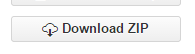
\includegraphics{git_zip.png}
\caption{The zipfile download button.}\label{intro:gitzip}\end{figure}

From the command line, navigate the newly extracted folder and use \code{pip} to
install the package. (In this case, \emph{path-to-gcmstools-folder} is the location
of the newly unzipped \emph{gcmstools} folder.)

\begin{Verbatim}[commandchars=\\\{\}]
home\PYGZgt{}\PYGZdl{} cd path\PYGZhy{}to\PYGZhy{}gcmstools\PYGZhy{}folder
gcmstools\PYGZgt{}\PYGZdl{} pip install .
\end{Verbatim}

\emph{Option 2 (recommended)}

First, install the \href{http://git-scm.com/}{version-control software Git}. Now, download and install
\emph{gcmstools} with one command.

\begin{Verbatim}[commandchars=\\\{\}]
home\PYGZgt{}\PYGZdl{} pip install git+https://github.com/rnelsonchem/gcms\PYGZus{}nnls.git
\end{Verbatim}

The advantage here is that the same command will update your \emph{gcmstools}
installation with any any changes that have been made to the main repository.

\emph{Uninstall}

Uninstallation of \emph{gcmstools} is identical regardless of the installation
method used above.

\begin{Verbatim}[commandchars=\\\{\}]
home\PYGZgt{}\PYGZdl{} pip uninstall gcmstools
\end{Verbatim}


\chapter{Basics of working with GCMS data files}
\label{basics:basics-of-working-with-gcms-data-files}\label{basics:version-control-software-git}\label{basics::doc}

\section{Export the data}
\label{basics:export-the-data}
First of all, be sure to export your GCMS data in a common data format, such
as \href{http://en.wikipedia.org/wiki/Mass\_spectrometry\_data\_format\#ANDI-MS\_or\_netCDF}{AIA, ANDI, or CDF.} It turns out that all of these formats \href{https://www.unidata.ucar.edu/support/help/MailArchives/netcdf/msg05748.html}{are related}
in that they are all based off of Network Common Data Format (\href{http://en.wikipedia.org/wiki/NetCDF}{netCDF}), so
they may have the file extension ``AIA'' or ``CDF''. This file type may not be the
default for your instrument, so consult the documentation for your GCMS
software to determine how to export your data in these formats.


\section{Set up the processing environment}
\label{basics:netcdf}\label{basics:set-up-the-processing-environment}
In order to process these files, run IPython from a terminal (command prompt
in Windows) in the folder containing the ``gcms.py'' file (which is the base
folder for this repository).  There are (at least) two ways to do this that
involve the command \code{cd} (change directory) run from either the terminal or
an IPython session. For example (\code{home\textgreater{}\$} is the command prompt located in
the folder ``home'', \code{In:} is the IPython prompt):

\begin{Verbatim}[commandchars=\\\{\}]
home\PYGZgt{}\PYGZdl{} ipython
In: \PYGZpc{}cd \PYGZdq{}path\PYGZhy{}to\PYGZhy{}gcms\PYGZhy{}folder\PYGZdq{}
Out: path\PYGZhy{}to\PYGZhy{}gcms\PYGZhy{}folder
In:
\end{Verbatim}

or:

\begin{Verbatim}[commandchars=\\\{\}]
home\PYGZgt{}\PYGZdl{} cd path\PYGZhy{}to\PYGZhy{}gcms\PYGZhy{}folder
gcms\PYGZgt{}\PYGZdl{} ipython
In:
\end{Verbatim}

The ``\emph{path-to-gcms-folder}'' is a valid path to the folder with ``gcms.py''. It
can take a little practice, but this gets easier very quickly. I'll assume you
use the second form of this as it makes using the \href{http://ipython.org/notebook.html}{IPython notebook} much
easier later.


\section{Read AIA data files}
\label{basics:ipython-notebook}\label{basics:read-aia-data-files}
First of all, you will need to \code{import} the ``gcms.py'' file to make the code
accessible to the IPython environment. This file contains a class called
\code{AIAFile} that reads and processes the GCMS files. AIAFile takes one
argument, which is a string with the file name. This string must have the path
(i.e.  folder) information if the file is not in the same directory as
``gcms.py''.  Sample data files are contained in a folder called ``data''.

\begin{Verbatim}[commandchars=\\\{\}]
In: import gcms
In: data = gcms.AIAFile(\PYGZsq{}data/datasample1.CDF\PYGZsq{})
\end{Verbatim}

The variable \code{data} now contains our processed GCMS data set. You can see
its contents using tab completion in IPython (\code{\textless{}tab\textgreater{}} refers to the tab
key).

\begin{Verbatim}[commandchars=\\\{\}]
In: data.\PYGZlt{}tab\PYGZgt{}
data.filename data.intensity data.nnls data.ref\PYGZus{}build data.times
data.integrate data.masses data.tic
\end{Verbatim}

All of these attributes are either data that describe or functions that modify
(methods) our dataset. You can inspect these attributes very easily in
IPython by just typing the name at the prompt.

\begin{Verbatim}[commandchars=\\\{\}]
In: data.times
Out:
array([0.08786667, ..., 49.8351])
In: data.tic
Out:
array([158521., ..., 0.])
\end{Verbatim}

This is a short description of these initial attributes:
\begin{itemize}
\item {} 
\emph{filename}: This is the name of the file that you imported.

\item {} 
\emph{times}: A Numpy array of the times that each MS was collected.

\item {} 
\emph{tic}: A Numpy array of the total ion chromatogram intensities.

\item {} 
\emph{masses}: A Numpy array the masses that cover the data collected by the MS.

\item {} 
\emph{intensity}: This is the 2D Numpy array of raw MS intensity data. The
columns correspond to the masses in the \code{masses} array and the rows
correspond to the times in the \code{times} array.

\end{itemize}

The remaining attributes \emph{ref\_build}, \emph{nnls}, and \emph{integrate} are functions
that deal with the non-negative fitting routine and are covered in later
sections.


\section{Simple plotting}
\label{basics:simple-plotting}
We can easily plot these data using the plotting package Matplotlib. As an
example, let's try plotting the total ion chromatogram. In this case,
\code{data.times} will be our ``x-axis'' data, and \code{data.tic} will be our ``y-axis''
data.

\begin{Verbatim}[commandchars=\\\{\}]
In: import matplotlib.pyplot as plt
In: plt.plot(data.times, data.tic)
Out:
[\PYGZlt{}matplotlib.lines.Line2D at 0x7f34\PYGZgt{}]
In: plt.show()
\end{Verbatim}

This should produce a pop-up window with an interactive plot, \hyperref[basics:ticplot]{Figure  \ref*{basics:ticplot}}.  (This should process should be fairly quick. However, sometimes
the plot initially appears behind the other windows, which makes it seem like
things are stuck. Be sure to scroll through your windows to find it.)
\begin{figure}[htbp]
\centering
\capstart

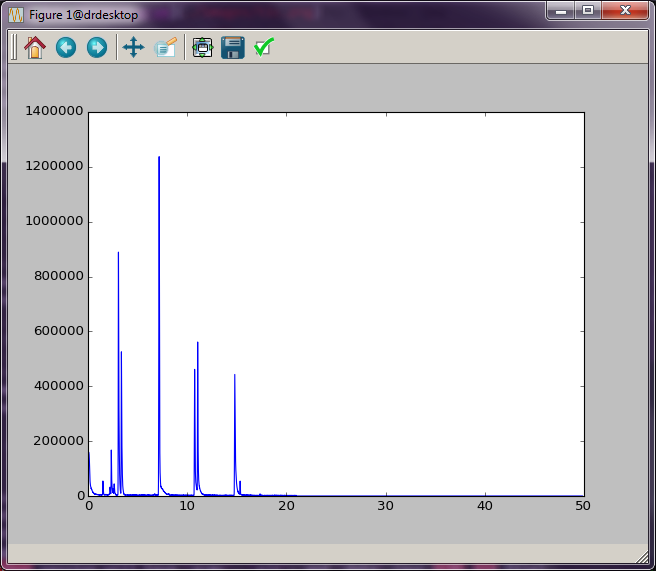
\includegraphics[width=3.5in]{tic.png}
\caption{Total ion chromatogram.}\label{basics:ticplot}\end{figure}

One drawback here is that you have to type these commands every time you want
to see this plot. There is another alternative, though. You can also put all
of these commands into a text file and run it with Python directly. Copy the
following code into a plain text file called ``tic\_plot.py''.

\textbf{NOTE}: it is very important that you are using a plain text file and not a
word processing (MS Word) document. On Mac/Linux, the ''.py'' suffix is not
required; however, in Windows, this suffix can be important. Unfortunately,
Windows hides file extentions by default, so you may have to search the web to
determine how to enable display of file extensions. Otherwise, you might end
up with a file called ``tic\_plot.py.txt'', which can work, but will most likely
cause confusion and annoyance. Anaconda ships with Spyder, a Python
development editor, which will take care of all of this for you, so you might
want to familiarize yourself with that program.

\begin{Verbatim}[commandchars=\\\{\}]
\PYG{k+kn}{import} \PYG{n+nn}{matplotlib.pyplot} \PYG{k+kn}{as} \PYG{n+nn}{plt}
\PYG{k+kn}{import} \PYG{n+nn}{gcms}

\PYG{n}{data} \PYG{o}{=} \PYG{n}{gcms}\PYG{o}{.}\PYG{n}{AIAFile}\PYG{p}{(}\PYG{l+s}{\PYGZsq{}}\PYG{l+s}{data/datasample1.CDF}\PYG{l+s}{\PYGZsq{}}\PYG{p}{)}
\PYG{n}{plt}\PYG{o}{.}\PYG{n}{plot}\PYG{p}{(}\PYG{n}{data}\PYG{o}{.}\PYG{n}{times}\PYG{p}{,} \PYG{n}{data}\PYG{o}{.}\PYG{n}{tic}\PYG{p}{)}
\PYG{n}{plt}\PYG{o}{.}\PYG{n}{show}\PYG{p}{(}\PYG{p}{)}
\end{Verbatim}

It is common practice to do all imports at the top of a Python program. That
way it is clear exactly what code is being brought into play. Run this new
file using the \code{python} command from the terminal.

\begin{Verbatim}[commandchars=\\\{\}]
gcms\PYGZgt{}\PYGZdl{} python tic\PYGZus{}plot.py
\end{Verbatim}

The window with your plot will now appear. (You will not be able to work in the
terminal until you close this window.) Alternatively, you can run this program
directly from IPython.

\begin{Verbatim}[commandchars=\\\{\}]
gcms\PYGZgt{}\PYGZdl{} ipython
In: \PYGZpc{}run tic\PYGZus{}plot.py
\end{Verbatim}

This also pops open a new window containing the interactive plot. It has the
advantage, however, that once the window is closed, you are dropped back into
an IPython session that ``remembers'' all of the variables and imports that you
created in your program file. In our example above, once the plot window is
closed, your IPython session will have \code{gcms}, \code{plt}, and \code{data} (our
GCMS AIA file) available.  This is very useful if you want to continue to work
interactively with your data, and it is a great way to remove a bunch of
repetitive typing.


\section{Working with multiple data sets}
\label{basics:working-with-multiple-data-sets}
In the example above, we opened our dataset into a variable called \code{data} in
order to be able to plot the TIC. If you want to manipulate more than one data
set, the procedure is exactly the same, except that you will need to use
different variable names for your other data sets.

\begin{Verbatim}[commandchars=\\\{\}]
In: data2 = gcms.AIAFile(\PYGZsq{}data/datasample2.CDF\PYGZsq{})
\end{Verbatim}

These two data sets can be plot together on the same figure by doing the
following:

\begin{Verbatim}[commandchars=\\\{\}]
In: plt.plot(data.times, data.tic)
Out:
[\PYGZlt{}matplotlib.lines.Line2D at 0x7f34\PYGZgt{}]
In: plt.plot(data2.times, data2.tic)
Out:
[\PYGZlt{}matplotlib.lines.Line2D at 0x02e3\PYGZgt{}]
In: plt.show()
\end{Verbatim}

The window shown in \hyperref[basics:twotic]{Figure  \ref*{basics:twotic}} should appear on the screen. (There
is a blue and green line here that are a little hard to see in this picture.
Zoom in on the plot to see the differences.)
\begin{figure}[htbp]
\centering
\capstart

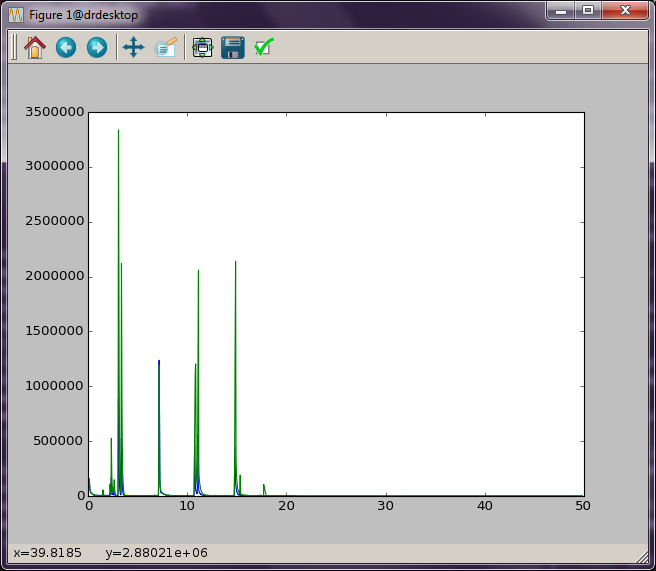
\includegraphics[width=3.5in]{tic2.png}
\caption{Two tic plotted together}\label{basics:twotic}\end{figure}


\chapter{Non-negative Least Squares Fitting}
\label{fitting:non-negative-least-squares-fitting}\label{fitting::doc}

\section{Collecting Reference MS Files}
\label{fitting:collecting-reference-ms-files}
A series of reference spectra are required if you want to do non-negative
least squares (NNLS) fitting of your data. There are two example files in this
repository to use as reference: ``ref\_spec.txt'' and ``ref\_spec2.MSL''. The MSL
file is a type of text file library that can be exported by programs like the
AMDIS or the NIST Mass Spectral Database. The .txt file was hand generated;
more information on this file format is provided in the next paragraph. The
format of both of these files is very important; however, MSL files are
typically autogenerated by external software and may not need manual
modification. A common feature of both formats, though, is that comment lines
can be included by starting a line with \code{\#}. This can be useful if you want
to add some notes or to remove reference spectra without deleting them
entirely.

Hand generated reference files must be text files that end with the prefix
''.txt''. Each reference compound must have at the minimum two labels: ``NAME''
and ``NUM PEAK''. ``NAME'' will be the reference name (probably want this to be
concise), and ``NUM PEAKS'' is followed by (at least) two space-separated
columns of MS data. The first column are m/z values, and the second column
are the intensity values. Intensities are normalized on import;
it is not necessary to do this by hand. Other labels can also be included if
you would like to incorporate extra metadata about the reference compound.
Each reference compound \emph{must} be separated by a blank line. Below is a small
sample of one of these files:

\begin{Verbatim}[commandchars=\\\{\}]
NAME:octane
FROM:www.massbank.jp
ID\PYGZus{}NUM: JP004695
NUM PEAKS:
  42 14.07 141
  43 99.99 999
  44 2.54 25
  45 4.03 40
  53 1.58 16
  55 19.83 198
  .
  .
  .
\end{Verbatim}

The online MS repository \href{http://www.massbank.jp/?lang=en}{massBank} is a useful place to find these mass and
intensity values. The data from that site is already formated correctly for
this file type.


\section{Loading Reference Spectra}
\label{fitting:loading-reference-spectra}\label{fitting:massbank}
In order to import this reference file, we will use the AIAFile object's
\code{ref\_build} function. Below is a repeat of the steps necessary in IPython to
set up our environment. (These are unchanged from the previous sections but are
repeated for clarity.)

\begin{Verbatim}[commandchars=\\\{\}]
In: import matplotlib.pyplot as plt
In: import gcms
In: data = gcms.AIAFile(\PYGZsq{}data/datasample1.CDF\PYGZsq{})
\end{Verbatim}

At this point, we are ready to read in our reference file using the function
\code{AIAFile.ref\_build}.


\chapter{Automated Calibration and Integration}
\label{calibration:automated-calibration-and-integration}\label{calibration::doc}

\section{Calibration Data}
\label{calibration:calibration-data}
If you have calibration data for a particular reference compound, you must
create a csv file and folder that have the same base name as the reference MS
file from above. Again, an examples are provided in this repository called
refcpd.csv and the folder refcpd. All of your calibration AIA files for this
compound need to be stored in the newly created folder. In order for these new
data files to be processed, the refcpd.csv file must be appropriately
modified.

The csv file is a simple comma-separated text file, but again the structure is
important. The first row in this file is critical. At the end, there are two
values that define the starting and stopping time points for integration.
Change these values based on the time range that you've determined from the
TIC of a calibration run. The rest of the rows are data file information.  The
first column is the name of a calibration data file, and the second column
needs to be the concentration of the reference compound associated with that
run. You don't have to add all of the calibration files here, but if they are
not in this list, they won't be processed.  Alternatively, any line that
starts with a `\#' is a comment, and will be ignored. In this way, you can
comment out samples, and add some notes as to why that sample was not used or
whatever.


\section{Run Calibrations}
\label{calibration:run-calibrations}
Once you've updated the calibration information from above. You can run the
program `calibration.py'. This runs through all of the reference spectra
defined in the `reference\_files.txt' file. If a `.csv' file exists for a
particular reference file, then a calibration will be performed.

All of the calibration data files listed in the csv file  will be processed
and a calibration curve generated. For each calibration sample, a plot of the
reference-extracted data will be generated in the calibration folder
(refcpd\_fits.png). In addition, a calibration curve plot is also generated
(refcpd\_cal\_curve.png'), which plots the integrated intensities and
calibrated intensities vs the concentrations. In addition, the calibration
information is printed on the graph for quick visual inspection. There is no
need to write down this calibration information.

This program has some important command line arguments that will change the
programs defaults. The first argument, `--nobkg', is a simple flag for
background fitting. By default, the fitting routine will select a MS slice
from the data set and use that as a background in the non-negative least
squares fitting. This procedure can change the integrated values. If you use
this flag, then a background MS will not be used in the fitting. Using a
background slice in the fitting may or may not give good results. It might be
a good idea to look at your data with and without the background subtraction
to see which is better.

The second command line argument is `--bkg\_time'. By default, the fitting
program uses the first MS slice as a background for fitting.  However, if
there is another time that looks like it might make a better background for
subtraction, then you can put that number here.

Here's a couple of example usages of this script:

\begin{Verbatim}[commandchars=\\\{\}]
\PYGZsh{} This will run the calibration program with all defaults
\PYGZdl{} python calibration.py
\PYGZsh{} This shuts off the background subtraction
\PYGZdl{} python calibration.py \PYGZhy{}\PYGZhy{}nobkg
\PYGZsh{} This sets an alternate time for the background subtraction
\PYGZsh{} In this case, the time is set to 0.12 minutes
\PYGZdl{} python calibration.py \PYGZhy{}\PYGZhy{}bkg\PYGZus{}time 0.12
\end{Verbatim}

Another file is also generated during this process: cal.h5. This is a HDF5
file that contains all of the calibration information for each standard. Do
not delete this file; it is essential for the next step. This is a very simple
file, and there are many tools for looking at the internals of an HDF5 file.
For example, \href{http://vitables.org/}{ViTables} is recommended. The background
information, such as whether a background was used and the time point to use
as a background spectrum, are stored as user attributes of the calibration
table.


\chapter{Process Sample Data}
\label{autoint:vitables}\label{autoint:process-sample-data}\label{autoint::doc}
Put all of your data files in a folder that must be called `data'. Once you've
done this, run the program `data.py' to process every AIA data file in that
folder using the calibration information that was determined from the steps
above.

This program opens the AIA file for the sample and performs non-negative least
squares analysis of the full data set using the reference spectra that are
listed in the `reference\_files.txt' file. Using the calibration information
that was determined above, it finds the concentrations of those components in
the sample data. For every reference compound that has associated calibration
information, a plot is generated that overlays the TIC (gray) and extracted
reference fit (blue). The title of the plot provides the calibrated
concentration information. Visual inspection of these files is recommended.

This file also accepts the same command line arguments as `calibration.py'
from the section above. You will be warned if you try to analyze your data
with different background information than the calibration samples. This may
not impact your data much, but it is good to know if you are doing something
different.

This file also generates another HDF5 file called `data.h5', which contains
the integration and concentration information for every component. This
information is identical to what is printed on the extraction plots above.
However, this tabular form of the data is a bit more convenient for comparing
many data sets. See the Calibration section for a recommended HDF5 file
viewer.



\renewcommand{\indexname}{Index}
\printindex
\end{document}
